\RequirePackage{ifpdf}
\documentclass[a4paper,11pt]{kth-bcs}
\usepackage[T1]{fontenc}
\usepackage{textcomp}
\usepackage{lmodern}
\usepackage[utf8]{inputenc}
\usepackage[swedish,english]{babel}
\usepackage{modifications}
\usepackage{url}
\usepackage{graphicx}

\usepackage[dvipdfm,bookmarks]{hyperref}

% use sane colors for hyperlinks
\usepackage{xcolor}
\definecolor{dark-red}{rgb}{0.4,0.15,0.15}
\definecolor{dark-blue}{rgb}{0.15,0.15,0.4}
\definecolor{medium-blue}{rgb}{0,0,0.5}
\hypersetup{
    colorlinks, linkcolor={dark-red},
    citecolor={dark-blue}, urlcolor={medium-blue}
}

% enable blank pages by:
% \afterpage{\blankpage}
\usepackage{afterpage}

\newcommand\blankpage{%
    \null
    \thispagestyle{empty}%
    \addtocounter{page}{-1}%
    \newpage}

% Define a new pagestyle called 'center'
\makepagestyle{center}
\makeevenfoot{center}{}{\thepage}{}
\makeoddfoot{center}{}{\thepage}{}

\DeclareGraphicsExtensions{.eps}
%\DeclareGraphicsExtensions{.png}

\title{Configuration and device identification on network gateways}

\subtitle{Konfigurering och enhetsidentifiering på nätverksgateways}
\foreigntitle{Konfigurering och enhetsidentifiering på nätverksgateways}
\author{Simon Kers}
\date{May 2013}
\blurb{Bachelor's Thesis at KTH\\
       School of Technology and Health\\
       Supervisor: Micael Lundvall\\
       Examiner: Ibrahim Orhan
%       Kungliga Tekniska Högskolan\\
%       Skolan för teknik och hälsa\\
%       136 40 Handen, Sweden\\
%       http://www.kth.se/sth
}

\trita{TRITA-STH 20XX:nn}

\begin{document}

\frontmatter
\pagenumbering{roman}
\setcounter{page}{3}
\pagestyle{center}

\maketitle
\thispagestyle{center}
\selectlanguage{english}
\begin{abstract}
   %why do we care about the problem?
To set up port forwarding rules on network gateways, certain technical skills are required from end-users.
These assumptions in the gateway software stack, can lead to an increase in support calls to the network operators and resellers of equipment, as well as a worsened user experience.
Other issues include faulty configuration, leaving the network vulnerable to attacks.
   %what did you actually do to get your results?

   %what did you learn/invent/create?
We present an enhancement of the web-based graphical user interface in the OpenWrt distribution, along with a wrapper for a network scanner, to detect devices and applications on the local network.
This relieves end-users of looking up forwarding rules for ports and protocols to configure their gateway, basing their decisions on data collected by the network scanner or by using an application name instead of its ports.

   %what are the larger implications of your findings
The implementation will reduce support costs for the service operators and improve the user experience.

\end{abstract}
\newpage
\blankpage

\begin{foreignabstract}{swedish}

\newpage
\blankpage

\end{foreignabstract}
\clearpage
\tableofcontents*
\mainmatter
\pagestyle{newchap}
\chapter{Introduction}
%brief introduction to inteno and the product
Inteno Broadband Technology is a company that supplies \emph{customer premises equipment} (CTE) for internet service providers.  
Their headquarters and research and development center is located in Stockholm, Sweden.
Inteno Open Systems Platform is a Linux-based open source platform running on customer premises equipment.
It is based on the OpenWrt distribution which targets embedded devices, specifically network gateways. \cite{Inteno}

%identified a real problem (motivate that it is real and interesting)
The technical support departments of partners and resellers of Intenos
customer premises equipment, are looking to reduce support costs and improve customer experience. 
Support issues creates costs for the business and by reducing the number of support tickets and their processing time, these costs can be reduced.

%come up with a solution (give a rough idea what the solution looks like)
By simplifying configuration through abstracting common tasks for the end-user, the number of support calls can be reduced.
Using automatic device identification and automating common tasks such as port forwarding, support costs can be reduced and end-user satisfaction is higher.
Many common support issues could be automated by the software running on the customer premises equipment and by effective communication with the end-user through the user interface.

%how I actually solved the problem (high-level summary of results).
The OpenWrt distribution provides a complete platform for compiling and
deploying a gateway firmware image.
By building a extensible library of presets for common port forwarding rules and developing a simple selection dialog, the amount of calls can be lowered while increasing customer satisfaction.

%skriv klart angående att tack vare ramverket så kan åf lägga till egna regler.


%\part{Important Results}

\chapter{Background}

Inteno produces hardware for customer premises equipment like network gateways and their direct customers are network operators and internet service providers.
The research and development department at Inteno works on improving the platform, adding value to the end users and the operators.

There are simple ways in which to improve the user experience, developers of network gateway software often implement a set of presets of port forwarding rules for common applications.
The interface presents the user with a list of applications in clear text and lets the user select an IP address, for which the forwarding rules should apply.

%skriv något om alternativa program typ port forwarding
Alternative solutions to simplifying port forwarding include using standalone applications which run on a PC, connected to the local network.
These applications has internal lists of port forwarding rules for common applications and devices, which is then applied for a specific IP address on the local network.
\cite{portforward.com}

%skriv något om alternativa program typ port scanner och guider på nätet
To test the newly applied configurations, web-based or locally run port scanners can be used.
They will scan the users external IP address for open ports and present which are open, this does not guarantee that the packets are routed to the correct internal address.

\section{Current situation}
The default settings page for port forwarding is currently located under the \emph{Firewall} tab, the forwarding procedure involves looking up ports for the specific device or unit.
These set of rules sometimes involve several ports and protocols, increasing the possibility for misstep and faulty configuration by the end user.
Such tasks are well suited for automation by the software suite, especially for applications and devices which require several port forwarding rules, automatic some of these steps will save time and bring overall value to the user experience.

\section{Software suite}

\subsection{OpenWrt}
OpenWrt is a free and open-source GNU/Linux distribution, targeting embedded devices, specifically wireless routers, but can run on almost any set of hardware.
Cross-compilation is enabled by OpenWrt Buildroot, which compiles the C code using uClibc, a lightweight C library focusing on embedded Linux systems. 
It intends to be a meta distribution and offers developers a framework on which to base their firmware on.

OpenWrt is generally compiled and linked using gcc and binutils, with the help of Makefiles and patches for the various gcc versions and target platforms.
Allowing end users as well as service operators and hardware manufacturers to compile the firmware.
It offers the BusyBox set of barebones UNIX tools, enabling advanced users to fully interact with their Linux system and providing developers with a familiar platform for debugging and testing their product.
\cite{OpenWrt:structure_design}

\subsection{OPKG}
The package management system used in OpenWrt is \emph{OPKG}. It is based off the discontinued \emph{ipkg} and operates similar to \emph{APT} and \emph{dpkg} of Debian-based distributions.
There are currently over 2000 OPKG packages available for OpenWrt.

The OpenWrt system and its packages are built using \emph{GNU Autoconf}.

\subsection{Inteno Open Platform System}
For Customer Premises Equipment\footnote{commonly abbreviated as CPE} like wireless gateways, Inteno Open Platform System offers an open-source Linux distribution based on OpenWrt.
It uses the OpenWrt build system including cross-compilation toolchain to ensure compatibility with the ecosystem and upstream.

\subsection{Lua Configuration Interface}
\emph{LuCI} is an suite of programs and libraries for extending OpenWrt using the Lua programming language.
It originated in the OpenWrt project but has since grown and is now it's own project.

The themes are accessed from the directory:

\begin{verbatim}
    root@Inteno:/usr/lib/lua/luci/view/themes/
\end{verbatim}

Rules for port forwarding are read from:

\begin{verbatim}
    /etc/config/firewall
\end{verbatim}

A port forwarding rule which forwards external HTTP traffic over port 80 to the local IP 192.168.1.214, as shown in \ref{fig:redirect_conf}.

foo: \ref{fig:foo}.


The presentation markup for the current port forwarding page in the LuCI backend on the Gateway, is defined in the file:

\begin{verbatim}
    luci-inteno/applications/luci-firewall/luasrc/view/firewall/cbi_addforward.htm

    libs/core/luasrc/model/firewall.lua :555
\end{verbatim}

in the functions:

\begin{verbatim}
    function redirect.*
\end{verbatim}

\chapter{Problem}
   \section{User experience}
Customers and operators of Inteno CPE have expressed concern about support costs for port forwarding and configuration in general.
The 

   \section{Support costs}

\chapter{Design}
   \section{Human-computer interaction}
This is a cite\cite{garrett2003elements}

   \section{Forwarding page}

See figure~\ref{fig:wizard-seq_dia} on page~\pageref{fig:wizard-seq_dia}.
\begin{figure}[h!]
   \centering
   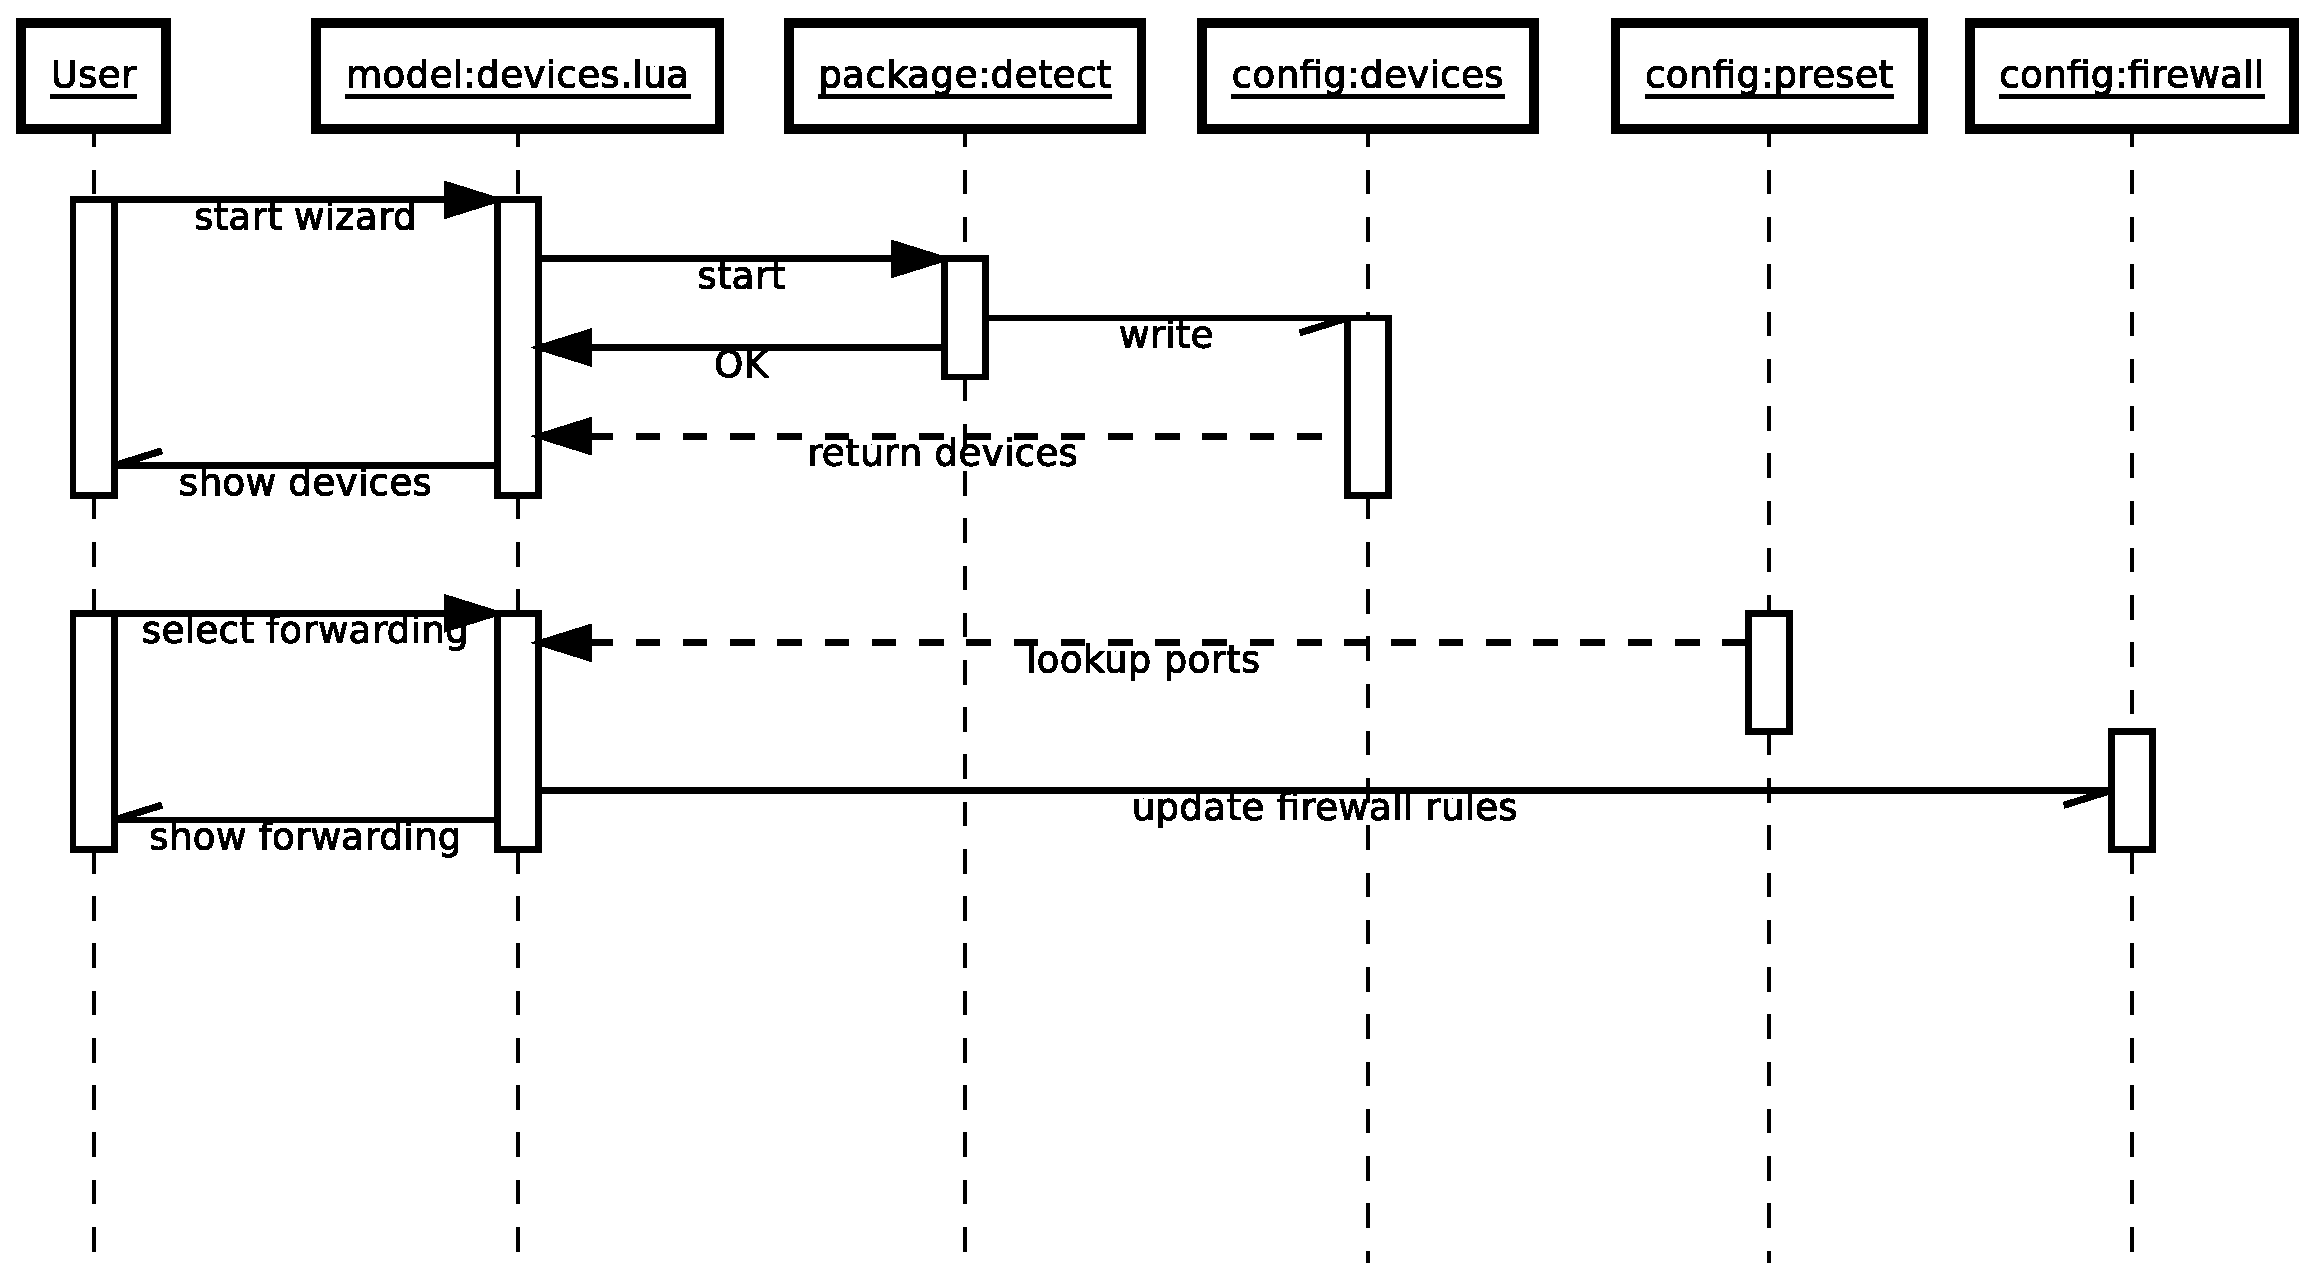
\includegraphics[width=15cm]{wizard-seq_dia}
   \caption{Sequential diagram of applying port forwarding rules}
   \label{fig:wizard-seq_dia}
\end{figure}

\chapter{Implementation}
%explain your approach in a general overview
The implementation consists of three general parts that work together in delivering easier forwarding rules configuration.
As shown in figure~\ref{fig:wizard-seq_dia}, the three configuration files that together with user input, are used as sources for the final redirection rule in the firewall configuration file.
The device detection updates the configuration file \emph{devices} with newly discovered devices, this does not include applications running on computers or game specific forwarding rules, running on gaming consoles, this requires user intervention.

%discuss tradeoffs, discuss traps you've fallen into

%explain your design and limitations in greater detail
Using the \emph{Unified Configuration System}, that is included in the OpenWrt distribution, all the basic commands for configuring the firewall rules were prototyped and explored.

\chapter{Results}
\section{Performance}

\chapter{Conclusions}
%discuss what we can learn from the results
Some text

%draw real conclusions

%explain how to fix shortcommings of work and how to fix them

\section{Further development}

\newpage
\newpage
\appendix
\addappheadtotoc
\chapter{Configuration files}\label{appA}
   %\addcontentsline{toc}{section}{Configuration files}
   \begin{figure}[ht]
      \centering
      \begin{verbatim}
config redirect               
        option target 'DNAT' 
        option src 'wan'
        option dest 'lan'
        option proto 'tcp'
        option src_dport '80'
        option dest_ip '192.168.1.214'
        option dest_port '80' 
        option name 'Web server'
      \end{verbatim}
      \caption{
         \small{
Port forwarding section in the \emph{firewall} configuration file
         }
      }
      \label{fig:redirect_conf}
   \end{figure}

   \begin{figure}[ht]
      \centering
      \label{fig:foo}
      \begin{verbatim}
         foo bar baz
      \end{verbatim}
      \caption{
         \small{
Port forwarding section in the \emph{firewall} configuration file
         }
      }
   \end{figure}
%\chapter{RDF}\label{appA}
%\begin{figure}[ht]
%   \begin{center}
%And here is a figure
%      \caption{
%         \small{
%            Several statements describing the same resource.
%         }
%      }
%      \label{RDF_4}
%   \end{center}
%\end{figure}
%
%that we refer to here: \ref{RDF_4}

\bibliographystyle{plain}
\bibliography{bibliography}
\end{document}
